\newpage
\section{Question 4}
	\subsection{Modified DH Notation}
	\noindent
	\begin{table}[position = here]
		\begin{centering}
			\begin{tabular}{||l|l|l|l|l||}
				\hline \rule[-2ex]{0pt}{5.5ex} \color{red}\bf{i} & \color{red}\bf{r}		&	\color{red}\bf{$\alpha$}	&	\color{red}\bf{d}	&	\color{red}\bf{$\theta$}\\ 
				\hline \rule[-2ex]{0pt}{5.5ex} 1 & 0	&	0		&	0		&	$\theta_{1}$\\	
				\hline \rule[-2ex]{0pt}{5.5ex} 2 & 0	&	$\pi/2$	&	0		&	$\theta_{1}$\\
				\hline \rule[-2ex]{0pt}{5.5ex} 3 & 10	&	$\pi/2$	&	0		&	$\theta_{1}$\\
				\hline \rule[-2ex]{0pt}{5.5ex} 4 & 12	&	$-\pi/2$&	0		&	$\theta_{4}$\\
				\hline \rule[-2ex]{0pt}{5.5ex} 5 & 0	&	$\pi/2$	&	10.5	&	$\theta_{1}$\\
				\hline 
			\end{tabular}\\
		\end{centering}
		\begin{flushleft}
			\caption [DHVariables] {Modified D-H Variable Notation}
		\end{flushleft}
	\end{table}
	
		\begin{figure}[position = here]
			\begin{centering}
				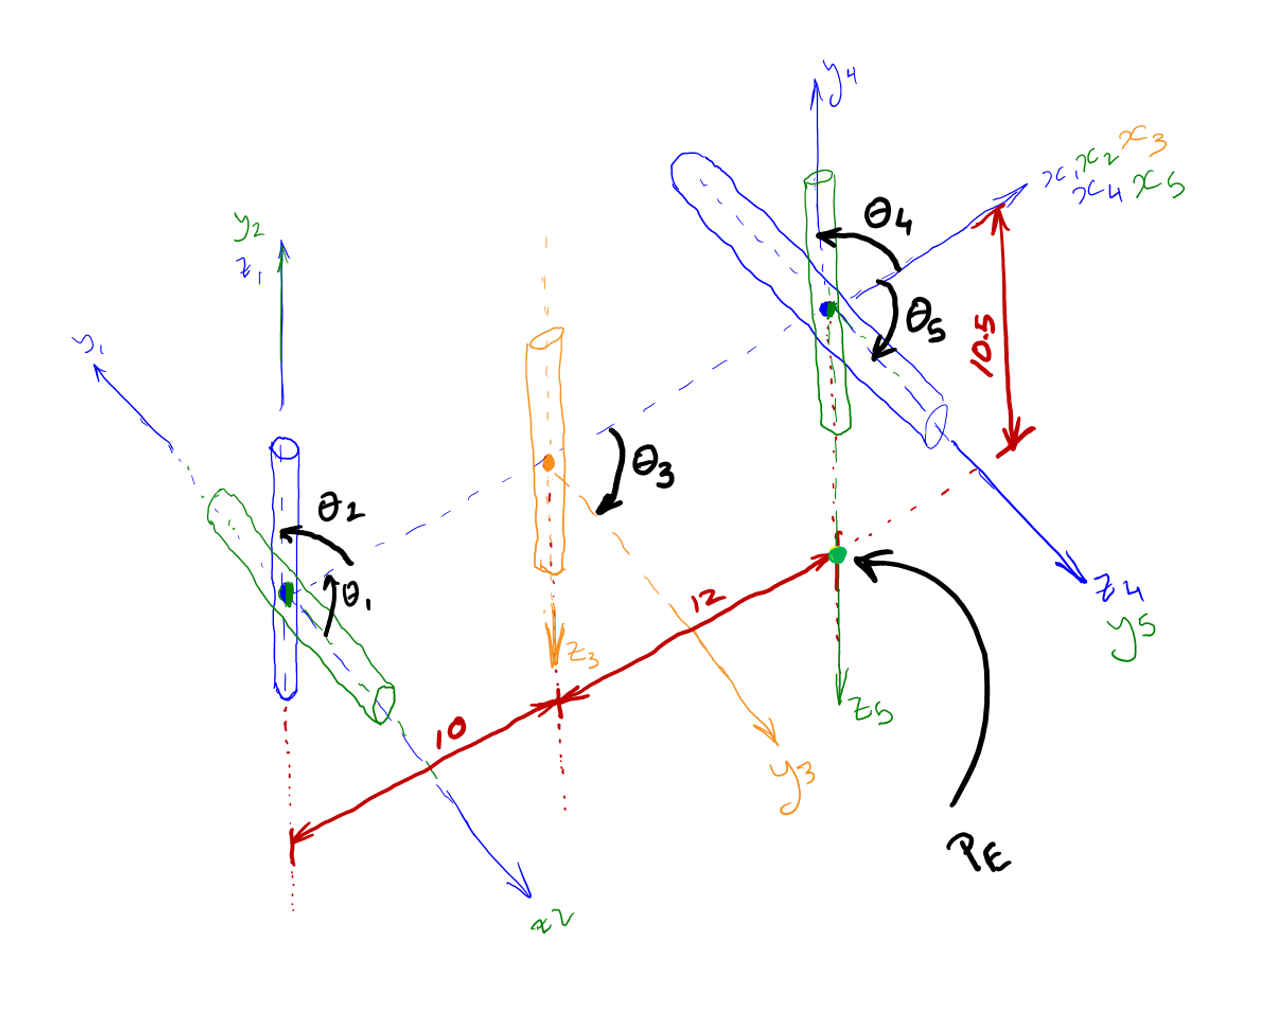
\includegraphics[scale=0.5]{q4Axes}\\
				\caption [DHDrawing]{Derived Coordinate Systems}
			\end{centering}
		\end{figure}
		
		\begin{figure}[position = here]
			\begin{centering}
				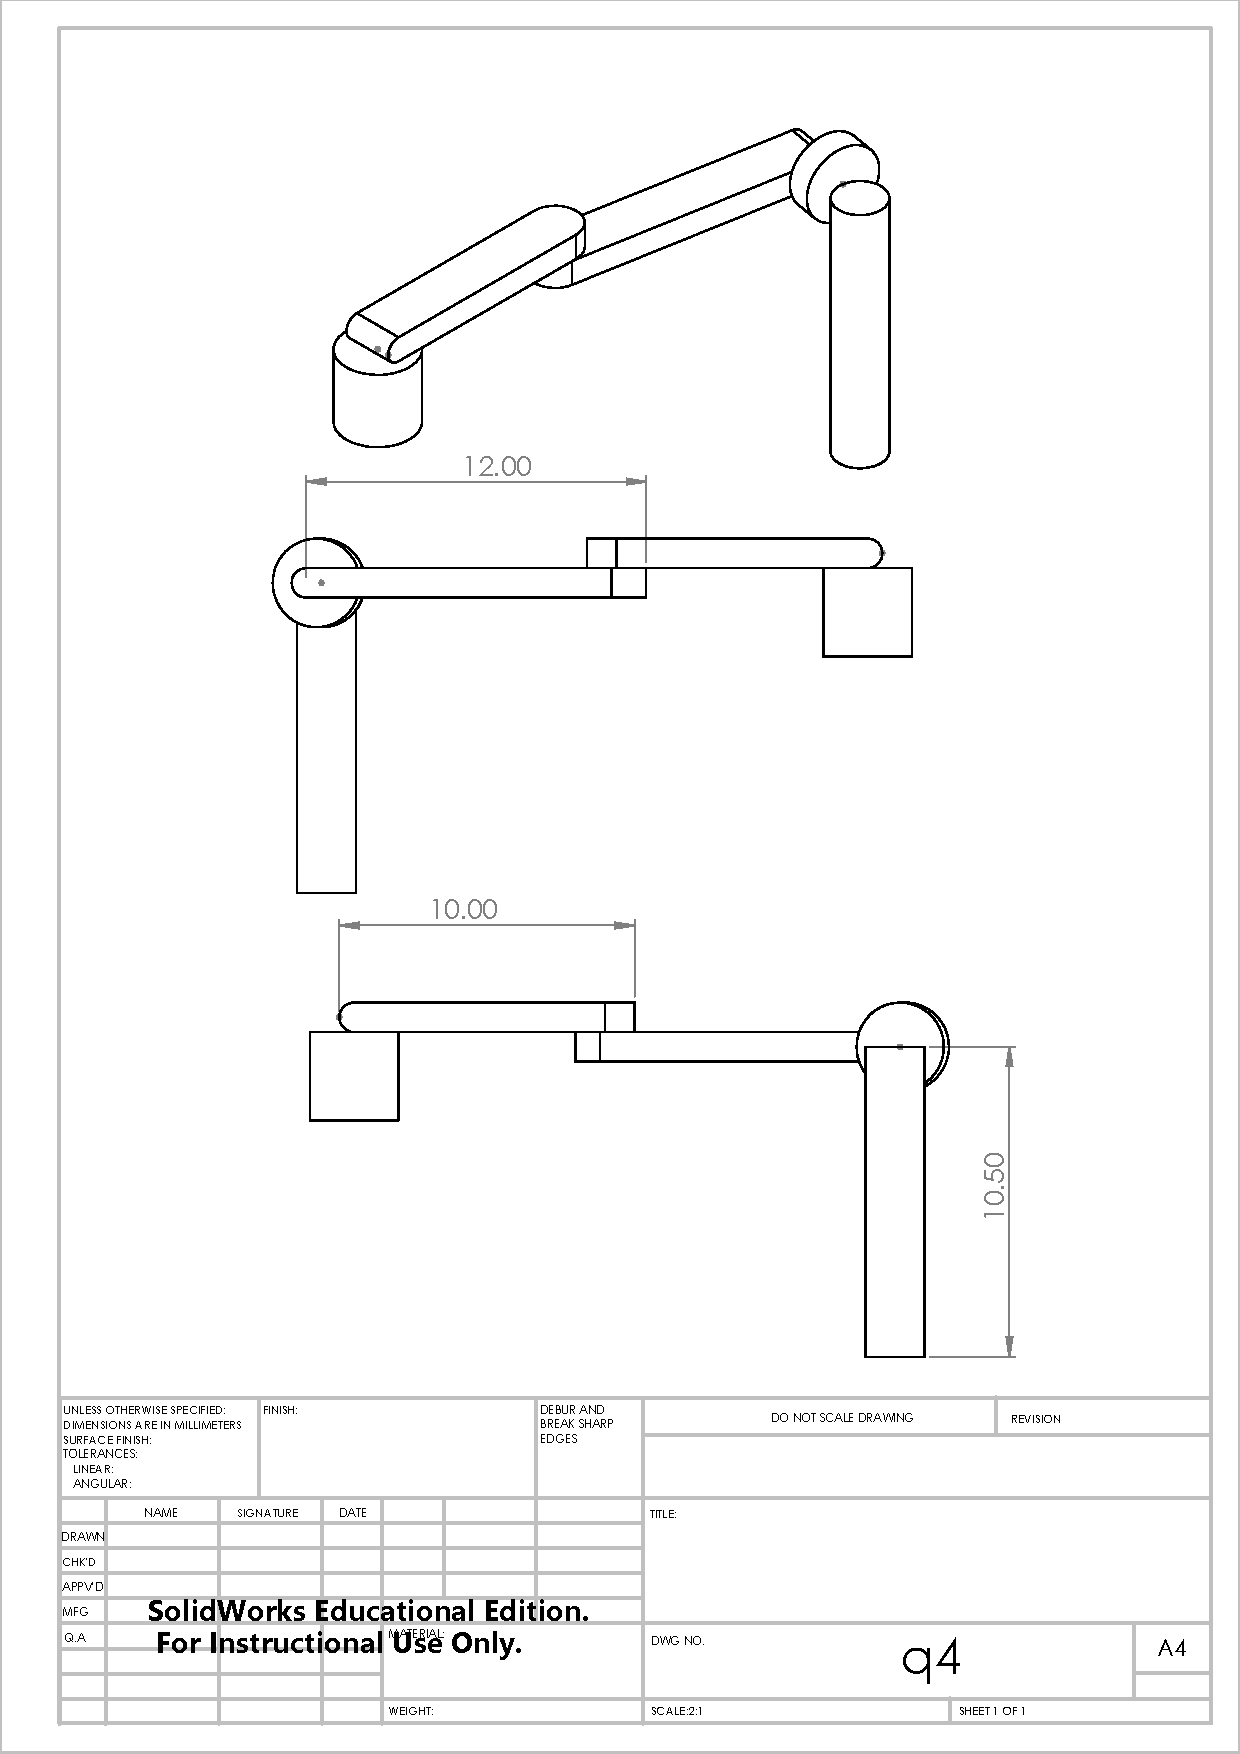
\includegraphics[scale=1.2]{q4}\\
				\caption [DHDrawing]{Derived Robot Arm Geometry}
			\end{centering}
		\end{figure}